\chapter{Longest common prefix array}\label{chapter:lcp}

A \emph{compressed suffix tree (CST)} is a compressed data structure that provides similar functionality as the concrete suffix tree. While the exact list of operations varies from proposal to proposal, the extra functionality over a suffix array (see Definition~\ref{def:suffix array}) is mostly tree navigation and determining the length of the longest common prefix of the suffixes in a given subtree. The majority of compressed suffix tree proposals are actually compressed enhanced suffix arrays, combining a CSA, a compressed representation of the LCP array, and some representation of the suffix tree topology \cite{Sadakane2007,Fischer2009a,Maekinen2010,Ohlebusch2009,Ohlebusch2010}.

In this chapter, we investigate compressed LCP array representations and their space-efficient construction, based on Paper~III. We describe a LCP array sampling mechanism that can be used in a similar way as the suffix array samples in a compressed suffix array. For regular texts, this representation offers better time/space trade-offs than the earlier compressed representations. We also describe an algorithm for constructing the LCP array directly from a compressed suffix array.


\section{LCP array representations}\label{sect:lcp representations}

In a plain representation of the LCP array, each element is a $\log n$\nobreakdash-bit integer, for a total of $n \log n$ bits. Yet as the array can be derived from the text, it should be at least as compressible as the text itself. A number of different compressed representations have been proposed for the LCP array. Most of them are based on one or more of the three main ideas: variable-length codes, storing the array in text order, and sampling the array.

\paragraph{Variable-length codes.}

If the text is not highly repetitive, most of the LCP values are likely to be small. An easy way to utilize this to compress the LCP array  is to store small values (less than $255$) as $8$\nobreakdash-bit integers \cite{Abouelhoda2004}. Large values are marked with a $255$ in the array and stored explicitly as pairs $(i, \LCP[i])$. If a large value is needed, it can be found efficiently with binary searching. On typical texts, where large LCP values are rare, this representation takes approximately $8n$ bits of space.

A more advanced representation \cite{Canovas2010} is based on directly addressable codes \cite{Brisaboa2009}. The binary representation of each LCP value is broken into $b$\nobreakdash-bit chunks. The $i$th element of array $B_{1}$ contains the least significant chunk of $\LCP[i]$, followed by a bit indicating whether more chunks are needed to encode the value. Array $B_{2}$ contains the next chunks of LCP values larger than $2^{b}-1$, and a \rank\ index is built over the indicator bits of array $B_{1}$ to map the elements of $B_{1}$ to the corresponding elements of $B_{2}$. If more than $2b$ bits needed to encode the largest LCP values, arrays $B_{3}, B_{4}, \dotsc$ are built in a similar way. On typical texts, this representation takes $6n$ to $8n$ bits of space, with an average access time similar to one \rank\ or \select\ operation on a bit vector.

\paragraph{Permuted LCP array.}

While encoding each LCP value individually allows fast random access, the compression results are not that good. For better compression, we have to encode the values relative to other values. The key to this is the \emph{permuted LCP (PLCP) array} $\PLCP$ that stores the LCP values in text order. By using the PLCP array and the suffix array, we can retrieve any LCP value as $\LCP[i] = \PLCP[\SA[i]]$.

\begin{definition}\label{def:left match}
For text $T[1,n]$ and integer $i > 1$, the \emph{left match} of suffix $T[\SA[i],n]$ is the suffix $T[\SA[i-1],n]$.
\end{definition}

It follows that $\PLCP[j]$ is the length of the longest common prefix of suffix $T[j,n]$ and its left match $T[j',n]$. As $\lcp(T[j'+1,n], T[j+1,n])$ is a lower bound for $\PLCP[j+1]$ (unless $\PLCP[j] = 0$), we get the following lemma.

\begin{lemma}[\cite{Kasai2001,Kaerkkaeinen2009}]\label{lemma:plcp}
For $j \in \set{1, \dotsc, n-1}$, $\PLCP[j+1] \ge \PLCP[j] - 1$.
\end{lemma}

The definition and the lemma generalize for collections of texts as well.

An immediate consequence of Lemma~\ref{lemma:plcp} is that values $\PLCP[j] + 2j$ form a strictly increasing sequence. Hence the PLCP array can be encoded as bit vector $B_{L}$ of length $2n$. Individual PLCP values can then be retrieved as $\PLCP[j] = \select_{1}(B_{L}, j) - 2j$. In the original proposal of Sadakane \cite{Sadakane2007}, bit vector $B_{L}$ was  a succinct bit vector with constant-time \select, taking $2n + o(n)$ bits of space and allowing constant-time access to individual PLCP values.

For highly repetitive texts, a run-length encoded bit vector representation of the PLCP array provides even better compression.

\begin{definition}\label{def:minimal plcp values}
A PLCP value $\PLCP[j]$ is \emph{minimal}, if $j = n$ or $\PLCP[j] < \PLCP[j+1] + 1$. Value $\PLCP[j]$ is \emph{maximal}, if $j = 1$ or $\PLCP[j-1]$ is minimal.
\end{definition}

In a maximal run of \onebit{}s in bit vector $B_{L}$, the first \onebit{} encodes a maximal PLCP value, and the last \onebit{} encodes a minimal value.

\begin{lemma}\label{lemma:non-minimal plcp values}
Value $\PLCP[j]$ is non-minimal if and only if $\PLCP[j] = \PLCP[j+1] + 1$.
\end{lemma}

\begin{proof}
By definition, $j < n$ and $\PLCP[j] \ge \PLCP[j+1] + 1$ for non-minimal $\PLCP[j]$. By Lemma~\ref{lemma:plcp}, $\PLCP[j] \le \PLCP[j+1] + 1$.
\end{proof}

\begin{lemma}\label{lemma:plcp run heads}
The \onebit{} encoding $\PLCP[\SA[i]]$ in bit vector $B_{L}$ can be a run head only if $\BWT[i]$ is also a run head.
\end{lemma}

\begin{proof}
Assume that $\BWT[i-1] = \BWT[i]$, and let $\SA[i-1] = j'$ and $\SA[i] = j$. Suffix $T[j',n]$ is then the left match of suffix $T[j,n]$. As we have $LF(i-1) = LF(i) - 1$, we also have that $T[j'-1,n] = T[\SA[LF(i-1)],n]$ is the left match of suffix $T[j-1,n] = T[\SA[LF(i)], n]$. And as $T[j'-1] = \BWT[i-1] = \BWT[i] = T[j-1]$, it follows that $\PLCP[j-1] = \PLCP[j] + 1$. As $\PLCP[j-1]$ is non-minimal by Lemma~\ref{lemma:non-minimal plcp values}, $\PLCP[j]$ is non-maximal, and the \onebit{} encoding $\PLCP[j]$ is not a run head.
\end{proof}

\begin{corollary}[\cite{Fischer2009a}]\label{corollary:plcp runs}
The number of runs of \onebit{}s in bit vector $B_{L}$ is at most $R$.
\end{corollary}

For every run of \onebit{}s, there is exactly one minimal and one maximal PLCP value. Note that $\PLCP[\SA[i]]$ is not necessarily a maximal value, when $\BWT[i]$ is a run head. Experimental results suggest that the number of runs of \onebit{}s in bit vector $B_{L}$ is usually about $2R/3$ (see Section~\ref{sect:lcp experiments}).

Proposed run-length encoded representations of bit vector $B_{L}$ require at most $2R \log (n/R) + O(R) + o(n)$ \cite{Fischer2009a} or $2R \log (n/R) + O(R \log \log (n/R))$ \cite{Maekinen2010} bits of space, and provide fast access to individual PLCP values. The main drawback of all PLCP-based representations is that when used with a compressed suffix array, accessing \emph{LCP} values requires using \locate, which is an expensive operation.

\paragraph{Sampled PLCP representations.}

An alternative way to compress the PLCP array is to sample one out of $d'$ values and use the text and the suffix array to derive the rest \cite{Khmelev2004}. Assume that we have sampled $\PLCP[ad']$ and $\PLCP[(a+1)d']$, and we want to determine $\PLCP[ad' + b]$ for some $b < q$. Lemma~\ref{lemma:plcp} states that $\PLCP[ad'] - b \le \PLCP[ad' + b] \le \PLCP[(a+1)d'] + d' - b$, so at most $d' + \PLCP[(a+1)d'] - \PLCP[ad']$ character comparisons are required to determine the missing value. While the number of comparisons can be large in the worst case, the average number of character comparisons over the array is $O(d')$ \cite{Kaerkkaeinen2009}.

With a more careful selection of the sampled positions, we get similar trade-offs even in the worst case. In particular, we can store the samples in $o(n)$ bits, while requiring only $O(\log^{\delta} n)$ character comparisons in the worst case, for any $\delta > 0$ \cite{Fischer2009}. This solution is essentially the \select\ structure of bit vector $B_{L}$ without the bit vector itself.

While the sampled PLCP representations provide attractive trade-offs when used with a plain suffix array, they are slow with a compressed suffix array. In addition to requiring the expensive \locate\ operation to access LCP values, they also use the equally expensive \extract\ for character comparisons.


\section{Sampling the LCP array}

While increasing the number of suffix array samples increases the performance of PLCP-based representations, it also quickly eliminates the size advantage of those representations. A sampled LCP representation can offer better time/space trade-offs, as individual LCP samples tend to be smaller than suffix array samples.

Assume that we have sampled the at most $R$ \emph{minimal} PLCP values, where $\PLCP[j] < \PLCP[j+1] + 1$. If we store these samples in suffix array order in the same way as suffix array samples, we can use a similar mechanism to retrieve the rest of the values. If $\LCP[i]$ has not been sampled, we proceed to position $\Psi(i)$ and check if $\LCP[\Psi(i)]$ has been sampled. If $\LCP[\Psi^{k}(i)]$ is the first sampled position we encounter, then $\LCP[i] = \LCP[\Psi^{k}(i)] + k$. This follows from the fact that $\LCP[\Psi^{k'}(i)]$ is a non-minimal PLCP value for all $k' < k$, and hence $\LCP[\Psi^{k'}(i)] = \PLCP[\SA[i] + k'] = \PLCP[\SA[i] + k' + 1] + 1 = \LCP[\Psi^{k'+1}(i)] + 1$ by Lemma~\ref{lemma:non-minimal plcp values}.

\begin{lemma}[\cite{Kaerkkaeinen2009}]\label{lemma:minimal plcp values}
For a text of length $n$, the sum of minimal or maximal PLCP values is at most $2n \log n$.
\end{lemma}

The worst case occurs in random texts, where most of the PLCP values are both maximal and minimal, and the average value is $\Theta(\log_{\sigma} n)$ (see the analysis in Section~\ref{sect:runs}). For a binary de Bruijn sequence, the sum of maximal values (with a looser definition, where Lemma~\ref{lemma:plcp run heads} holds in both directions) is $(n/2) \log n - O(n)$ \cite{Kaerkkaeinen2009}, making the bound asymptotically tight. In highly repetitive texts, the sum of minimal values tends to be less than $n$ (see Section~\ref{sect:lcp experiments}).

If we use the bit vector of Gupta \etal{Gupta2007} to mark the sampled positions, the vector takes $(1 + O(1 / \log R)) R \log (n/R) + O(R \log \log (n / R))$ bits of space in the worst case. As the sum of the samples is at most $2n \log n$, we can concatenate the binary representations of the samples in at most $R \log (2n \log n / R) + R$ bits. The two-level storage scheme of Ferragina and Venturini \cite{Ferragina2007} allows constant-time access to the samples by using $O(R \log \log n / \log n)$ bits of extra space. Overall, the samples require
$$
\left( 2 + O\left( \frac{1}{\log R} \right) \right) R \log \frac{n}{R} +
O\left( R \log \log \frac{n}{R} \right)
$$
bits of space, which is almost the same as for one of the run-length encoded PLCP proposals \cite{Maekinen2010}.

To guarantee worst-case behavior and to improve the performance with highly repetitive texts, where $R \ll n$, we also sample one out of $d' > 0$ PLCP values, when the successive minimal values are spaced more than $d'$ positions apart. With the pessimistic assumption that each of these extra samples is large, requiring $\log n$ bits, the size bound becomes
$$
\left( 1 + O\left( \frac{1}{\log n_{S}} \right) \right) n_{S} \log \frac{n}{n_{S}} +
R \log \frac{n}{R} +
\frac{n \log n}{d'} +
O\left( n_{S} \log \log \frac{n}{n_{S}} \right)
$$
bits, where $n_{S} \le R + n/d'$ is the number of samples. In practice, an extra sample $\PLCP[j]$ requires roughly $\log \PLCP[j]$ bits and a mark in the bit vector, while an extra suffix array sample requires $2 \log (n/d)$ bits in addition to the mark, where $d$ is the suffix array sample rate. Hence with typical sample rates, adding extra LCP samples is cheaper than adding the same number of suffix array samples.

\begin{theorem}\label{theorem:sampled lcp}
Let $T[1,n]$ be a text, and let $d' > 0$ be an integer. The LCP samples for text $T$ with sample rate $d'$ require
$$
O\left(  n_{S} \log \frac{n}{n_{S}} \right) + \frac{n \log n}{d'}
$$
bits of space, where $n_{S} \le R + n/d'$ is the number of samples, and $R$ is the number of equal letter runs in the Burrows-Wheeler transform of text $T$. A compressed suffix array that computes $\Psi$ in $t_{\Psi}$ time can use the samples to access any element of the LCP array in $O(d' \cdot (t_{\Psi} + o(\log n)))$ time.
\end{theorem}


\section{Space-efficient LCP array construction}

Kasai \etal{Kasai2001} introduced the first linear-time LCP array construction algorithm. As the algorithm requires the suffix array in memory, it uses $\Theta(n \log n)$ bits of space for a text of length $n$. Yet as the LCP array can be compressed into $2n + o(n)$ bits or even less, this greatly restricts the size of the texts with which the LCP array can be used. Later developments concentrated on reducing the working space to $O(n \log \sigma)$ bits \cite{Puglisi2008,Kaerkkaeinen2009,Gog2011,Beller2011} or making the construction faster in practice \cite{Kaerkkaeinen2009,Gog2011,Fischer2011}.

The fastest algorithm so far is the one by Fischer \cite{Fischer2011}. Based on a suffix array construction algorithm using induced sorting \cite{Nong2009a}, the algorithm works in linear time, yet requires $\Theta(n \log n)$ bits of working space. Another interesting algorithm is the one by Beller \etal{Beller2011} that builds the LCP array directly from a compressed suffix array. On a conceptual level, the algorithm is based on repeating the following for $k = 0, 1, \dotsc$.

\begin{enumerate}

\item For all patterns $P$ of length $k$, let $[sp_{P}, ep_{P}]$ be the suffix array range containing the occurrences of the pattern. Assume that set $Q_{k}$ contains all these ranges.

\item Use backward searching to determine set $Q_{k+1}$ from set $Q_{k}$.

\item For each range $[sp, ep] \in Q_{k+1}$, set $\LCP[ep+1] \leftarrow k$, unless $\LCP[ep+1]$ has already been defined.

\end{enumerate}

A practical variant of the algorithm works in $O(n \log n)$ time and uses roughly $n$ bytes of working space in addition to the compressed suffix array. The LCP array is written directly to disk in several passes. While the algorithm is reasonably fast and space-efficient, it cannot be used for constructing the LCP array for texts that are too large to fit into memory. This is in contrast to the compressed suffix arrays, for which such algorithms exist (see Chapter~\ref{chapter:construction}).

By starting from the \emph{irreducible LCP algorithm} of Kärkkäinen \etal{Kaerkkaeinen2009}, we can design an LCP array construction algorithm that uses negligible working space in addition to the compressed suffix array and the compressed (P)LCP representation. The irreducible LCP algorithm finds the irreducible (maximal) PLCP values, computes them directly, and uses Lemma~\ref{lemma:non-minimal plcp values} to derive the rest of the values. As the sum of maximal PLCP values is at most $2n \log n$, the algorithm works in $O(n \log n)$ time. The PLCP values are computed in text order, making it possible to build any compressed PLCP representation directly.

The original irreducible LCP algorithm uses the text and the suffix array to identify the maximal values. With a compressed suffix array, we want to identify the irreducible values using function $\Psi$ in one pass over the text. Additionally, as computing the irreducible values also involves scanning the text forward using $\Psi$, we can avoid redundant work by finding minimal instead of maximal PLCP values.

From Lemma~\ref{lemma:plcp run heads}, we can derive the following result by noting that $\PLCP[j]$ is minimal if $\PLCP[j+1]$ is maximal.

\begin{lemma}\label{lemma:identifying minimal plcp values}
Let $\SA[i] = j$. Value $\PLCP[j]$ can be minimal only if $j = n$ or if $\BWT[\Psi(i)]$ is a run head.
\end{lemma}

Let $c$ be a character such that $C[c] < i \le C[c+1]$. As we compute $\Psi(i) = \mselect_{c}(\BWT, i - C[c])$, we know that $\BWT[\Psi(i)]$ is a run head if we use a run head in $\BWT$ (or in bit vector $B_{c}$) to compute $\Psi(i)$. Equivalently, $\BWT[\Psi(i)]$ is a run head if and only if $\mchar(i-1) \ne \mchar(i)$ or $\Psi(i-1) \ne \Psi(i) - 1$.

While Lemma~\ref{lemma:identifying minimal plcp values} produces false positives, we can identify true minimal values by buffering the previous candidate, until we find the next possibly minimal value. The modified irreducible LCP algorithm can be seen in Figure~\ref{fig:irreducible lcp algorithm}.

\begin{figure}
\begin{tabbing}
mm\=mm\=mm\=mm\= \kill
\> \textbf{function} $\lcp(i)$ \\
\> \> $(i', k) \leftarrow (i-1, 0)$ \\
\> \> $c \leftarrow \mchar(i)$ \\
\> \> \textbf{while} $i' \in C_{c}$ \\
\> \> \> $(i', i, k) \leftarrow (\Psi(i'), \Psi(i), k + 1)$ \\
\> \> \> $c \leftarrow \mchar(i)$ \\
\> \> \textbf{return} $k$ \\
\\
\> \textbf{function} $\operatorname{irreducibleLCP}(\SA^{-1}[1])$ \\
\> \> $\PLCP[1] \leftarrow 0$ \\
\> \> $(i, j, j') \leftarrow (\SA^{-1}[1], 1, 2)$ \\
\> \> \textbf{while} $j < n$ \\
\> \> \> $c \leftarrow \mchar(i)$ \\
\> \> \> \textbf{if} $i-1 \not\in C_{c}$ \textbf{or} $\Psi(i-1) \ne \Psi(i) - 1$ \\
\> \> \> \> $x \leftarrow \lcp(\Psi(i))$ \\
\> \> \> \> $\PLCP[j', j+1] \leftarrow (x + j+1 - j', \dotsc, x)$ \\
\> \> \> \> $j' \leftarrow j + 2$ \\
\> \> \> $(i, j) \leftarrow (\Psi(i), j + 1)$ \\
\> \> \textbf{return} $\PLCP$ 
\end{tabbing}

\caption{The irreducible LCP algorithm for computing the PLCP array directly from a compressed suffix array. The algorithm maintains an invariant that $\SA[i] = j$, while $\PLCP[j']$ is the maximal value in the current run.}\label{fig:irreducible lcp algorithm}
\end{figure}

A two-pass variant of the same algorithm can be used to sample the LCP array. In the first pass, we scan the CSA in suffix array order, and find the minimal samples. As the samples are output in suffix array order, we can compress them immediately, using negligible working space. The second pass is in text order, as in the original algorithm. We output one out of $d'$ consecutive non-minimal values as pairs $(i, \LCP[i])$, deriving $\LCP[i]$ from the next sample. Once the non-minimal samples have been determined, we sort them in suffix array order, and merge them with the minimal samples.

\begin{theorem}\label{theorem:irreducible lcp algorithm}
Given a compressed suffix array for a text of length $n$, the irreducible LCP algorithm computes the PLCP array in negligible working space in addition to the CSA and the PLCP array. The running time of the algorithm is equivalent to extracting $O(n \log n)$ characters from the text using the CSA. A two-pass version of the algorithm samples the LCP array with sample rate $d' > 0$ in the same time bound, while using $O((n/d') \log n)$ bits of additional working space.
\end{theorem}
\newpage


\section{Implementation and experiments}\label{sect:lcp experiments}

LCP samples, bit vector encodings of the PLCP array, and their construction algorithms have been implemented as a part of RLCSA (see Chapter~\ref{chapter:rlcsa}). For PLCP, we use a run-length encoded bit vector with highly repetitive data sets, and a succinct bit vector with regular data sets. For marking the sampled LCP positions, we similarly use a gap encoded bit vector with highly repetitive data sets, and a succinct vector with the regular ones. The sampled values are encoded with \deltacode{}s, and stored in a stripped-down version of the gap encoded bit vector for fast access.

The succinct bit vector is a practical implementation designed for current hardware. For \rank, we divide the vector into $256$\nobreakdash-bit blocks, and store the number of \onebit{}s before each block in $\log n$ bits. Solving \rank{} then requires retrieving the stored value for the correct block, and counting the number of $1$-bits in the block up to the queried position using the $64$-bit $\popcount$ function provided in GCC. The function compiles either into a single instruction or a small subroutine, depending on architecture.

For \select, the implementation uses two levels of indexes. The first one stores $n/256$ pointers to blocks that contain the \onebit{} of rank $i \cdot 256n_{1}/n + 1$, for $i = 0$ to $n/256 - 1$. With this index, we get a range of blocks that contains the queried \onebit. If the range spans more than $16$ blocks, we use binary search in the \rank{} index to narrow it down. When the range becomes short enough, we continue with linear search in the \rank{} index to find the correct block, and resort to $\popcount$ to compute the answer within the block.

To avoid redundant work in LCP sampling and PLCP construction, we interleave the computation of minimal values with the main loop. When sampling the LCP array, we make both of the passes in text order, and store all samples in an array of pairs $(i, \LCP[i])$ before compressing them.

For the experiments, we used the same system as in Section~\ref{sect:rlcsa experiments}. Only once core was used in the experiments. We used the same four data sets as in Paper~III. As regular data sets, we used human DNA sequences (dna) and English language texts (english) from the Pizza \& Chili Corpus \cite{Ferragina2009a}. As highly repetitive data sets, we used Finnish language Wikipedia with full version history (fiwiki) and the genomes of 36 strains of \emph{Saccharomyces paradoxus} (para) (see also Chapter~\ref{chapter:rlcsa}). When the data set was much larger than 400 megabytes, a 400 MB prefix was used instead. Further information on the data sets can be found in Table~\ref{table:lcp data sets}.

\begin{table}
\centering
\renewcommand{\tabcolsep}{.1cm}
\begin{tabular}{lccccccccc}
\hline\noalign{\smallskip}
 & & & & \multicolumn{2}{c}{\textbf{Minimal}} & & \multicolumn{3}{c}{\textbf{Construction}} \\
\textbf{Data set} & \textbf{Size} & \textbf{Runs} & & \textbf{Number} & \textbf{Sum} & & \textbf{PLCP} & \textbf{Samples} & \textbf{Induced} \\
\noalign{\smallskip}
\hline
\noalign{\smallskip}
dna     & 385 & 243.49 & & 158.55 & 2215 & & 2402 & 2695 & 47 \\
english & 400 & 156.35 & &  99.26 & 1052 & & 1181 & 1471 & 76 \\
fiwiki  & 400 &   1.79 & &   1.15 &  117 & &  210 &  365 & 46 \\
para    & 409 &  15.64 & &  10.05 &  299 & &  374 &  590 & 55 \\
\noalign{\smallskip}
\hline
\end{tabular}

\caption{Data sets used in LCP experiments. Size in megabytes, millions of runs in BWT, number and sum of minimal samples in millions, and construction time in seconds. Construction times for PLCP and (LCP) Samples are from using the irreducible LCP algorithm, while Induced is for building the LCP array with the algorithm of Fischer \cite{Fischer2011}, which is currently the fastest LCP construction algorithm.}\label{table:lcp data sets}
\end{table}

The construction times reported in Table~\ref{table:lcp data sets} are for the highest number of SA and LCP samples. Note that sample rates had no significant impact on construction times. With the regular data sets, the irreducible LCP algorithm was very slow, as its time complexity scales with the sum of minimal PLCP values. A parallel version that scans different sequences in different threads might still be as fast as direct CSA construction (see Chapter~\ref{chapter:construction}), as the basic CSA operations parallelize well. The algorithm was much faster with the highly repetitive data sets, while still being $5$ to $10$ times slower than the LCP construction algorithm of Fischer \cite{Fischer2011}.

As noted in Section~\ref{sect:lcp representations}, the number of minimal PLCP values was roughly $2/3$ times the number of equal letter runs in the Burrows-Wheeler transform of the text. As the number of minimal PCLP values is the same as the number of runs of \onebit{}s in the PLCP vector $B_{L}$, this means that the size bounds for the run-length encoded PLCP variants are significantly larger than the size in practice.

To compare the time/space trade-offs offered by PLCP bit vectors and LCP samples, we built RLCSA with sample rates $d = 8, 16, 32, 64$ for the regular data sets, and $d = 32, 64, 128, 256$ for the highly repetitive data sets. We used LCP sample rates $d' = 8, 16$ for the regular data sets, and $d' = 16, 32, 64$ for the highly repetitive ones. Instead of measuring the average time required for a random LCP query, we used a measure that is independent of the underlying CSA implementation, counting the average number of steps of $\Psi$ required to find a sampled SA or LCP position. The results can be seen in Figure~\ref{fig:lcp results}. As a lower bound for the size of any PLCP-based representation, we also included the results for \locate{} in the figures.

\begin{figure}
\centerline{
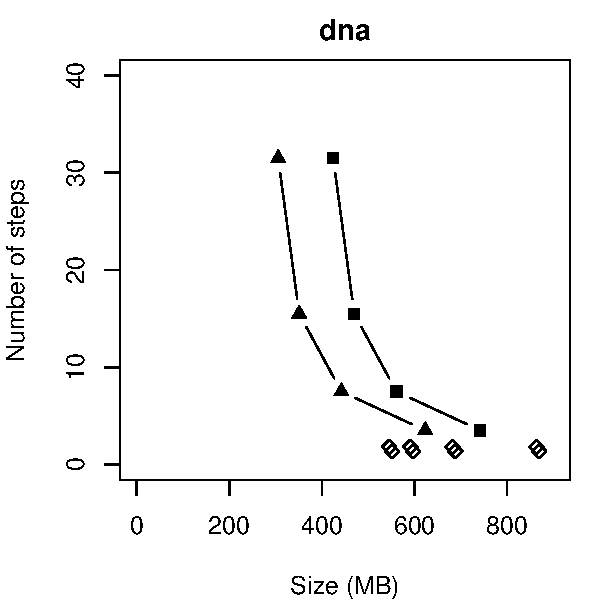
\includegraphics[width=.45\textwidth]{experiments/lcp/dna.pdf}
\hspace{5pt}
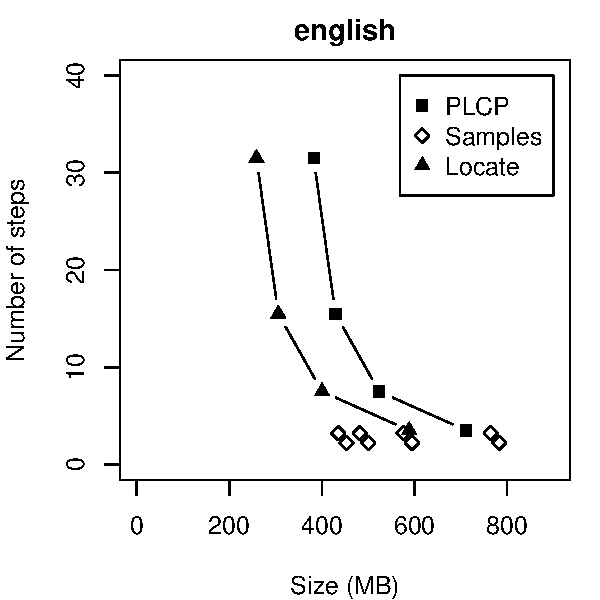
\includegraphics[width=.45\textwidth]{experiments/lcp/english.pdf}}

\centerline{
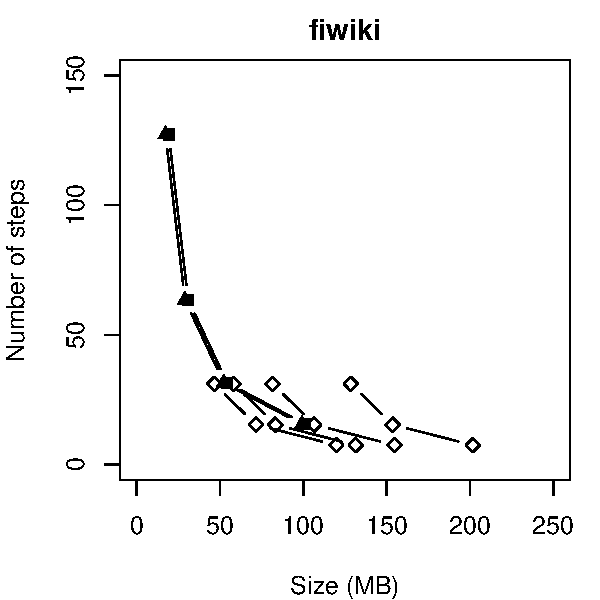
\includegraphics[width=.45\textwidth]{experiments/lcp/fiwiki.pdf}
\hspace{5pt}
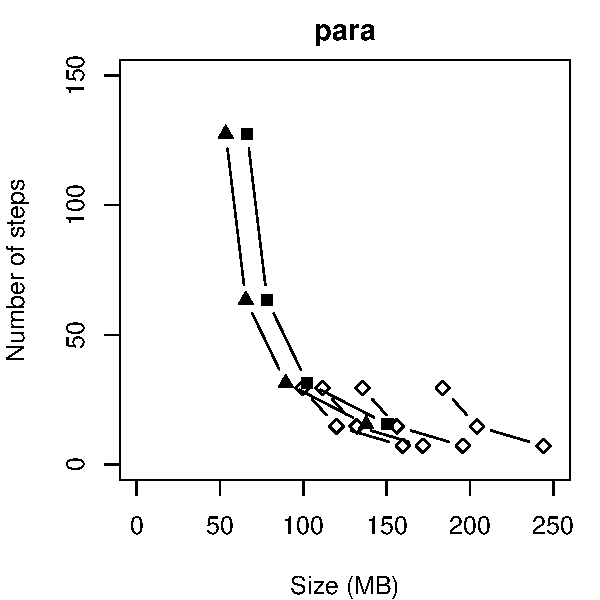
\includegraphics[width=.45\textwidth]{experiments/lcp/para.pdf}
}
\caption{Experimental results for $10^{6}$ random LCP queries with LCP samples and PLCP, with $10^{6}$ random \locate{} queries as a lower bound for any PLCP-based representation. Index size in megabytes and the average number of steps required to reach a SA/LCP sample. The results with LCP samples have been grouped by SA sample rate.}
\label{fig:lcp results}
\end{figure}

With the regular data sets and sparse SA sampling, the performance of LCP samples was superior to the PLCP-based approach, while increasing the overall index size only slightly. As $25\%$ (english) to $40\%$ (dna) of text positions were sampled, a sampled position was found in a couple of steps most of the time. With denser suffix array sampling, this advantage mostly disappeared, as the \locate{} queries were no longer that expensive.

As there were only a few minimal samples in the highly repetitive data sets (see Table~\ref{table:lcp data sets}), the solution using LCP samples relied mostly on the non-minimal extra samples. This made the LCP samples significantly larger than the run-length encoded PLCP bit vector. While the LCP samples still offered better time/space trade-offs than any PLCP-based approach in some cases, the improvement was not significantly better than what could be achieved by denser suffix array sampling.

We also measured the average number of steps required for computing the LCP values directly. As there were long repetitions even in the regular data sets, the results (2424 steps in dna and 5786 steps in english) were not competitive with the other approaches. Still, as many of the minimal samples are small, it should be possible to decrease the size of the samples without sacrificing too much performance by storing only large minimal samples, and computing the small ones directly when required.
